\documentclass[10pt]{article}
\usepackage[margin=.7in]{geometry}
\usepackage[T1]{fontenc}
%\usepackage{amsmath,amssymb,amsthm}
%\usepackage{enumerate}
%\usepackage{minibox}
%\usepackage[table]{xcolor}

\usepackage{csvsimple}
\usepackage{booktabs}
\usepackage{tikz}
\usepackage{pgfplots}

\usepackage{underscore}

\pgfplotsset{width=12cm,compat=1.3}

% \def\code#1{\texttt{#1}}

%%%%%%%%%%%%%%%%%%%%%%%%%%%%%%%%%%%%%%%%%%%%%%%%%%%%%%%%%%%%%%%%%%%%%%%%%
\title{CSCE 313.506-F18: \\Programming Assignment 5}
\author{Tristan Seifert}
\date{Due: Sunday, Nov. 11, 2018}

%%%%%%%%%%%%%%%%%%%%%%%%%%%%%%%%%%%%%%%%%%%%%%%%%%%%%%%%%%%%%%%%%%%%%%%%%
\begin{document}
\maketitle

\hrule

%%%%%%%%%%%%%%%%%%%%%%%%%%%%%%%%%%%%%%%%%%%%%%%%%%%%%%%%%%%%%%%%%%%%%%%%%
\section{Performance Data}
This data was gathered for varying values of $w$ and $b$ while $n = 10000$. The system used runs macOS 10.14.2, with 64GB of RAM and dual Xeon E5-2670 v2 (10 physical cores, 20 virtual cores) processors at 2.6 GHz.

\begin{figure}[h]
\centering
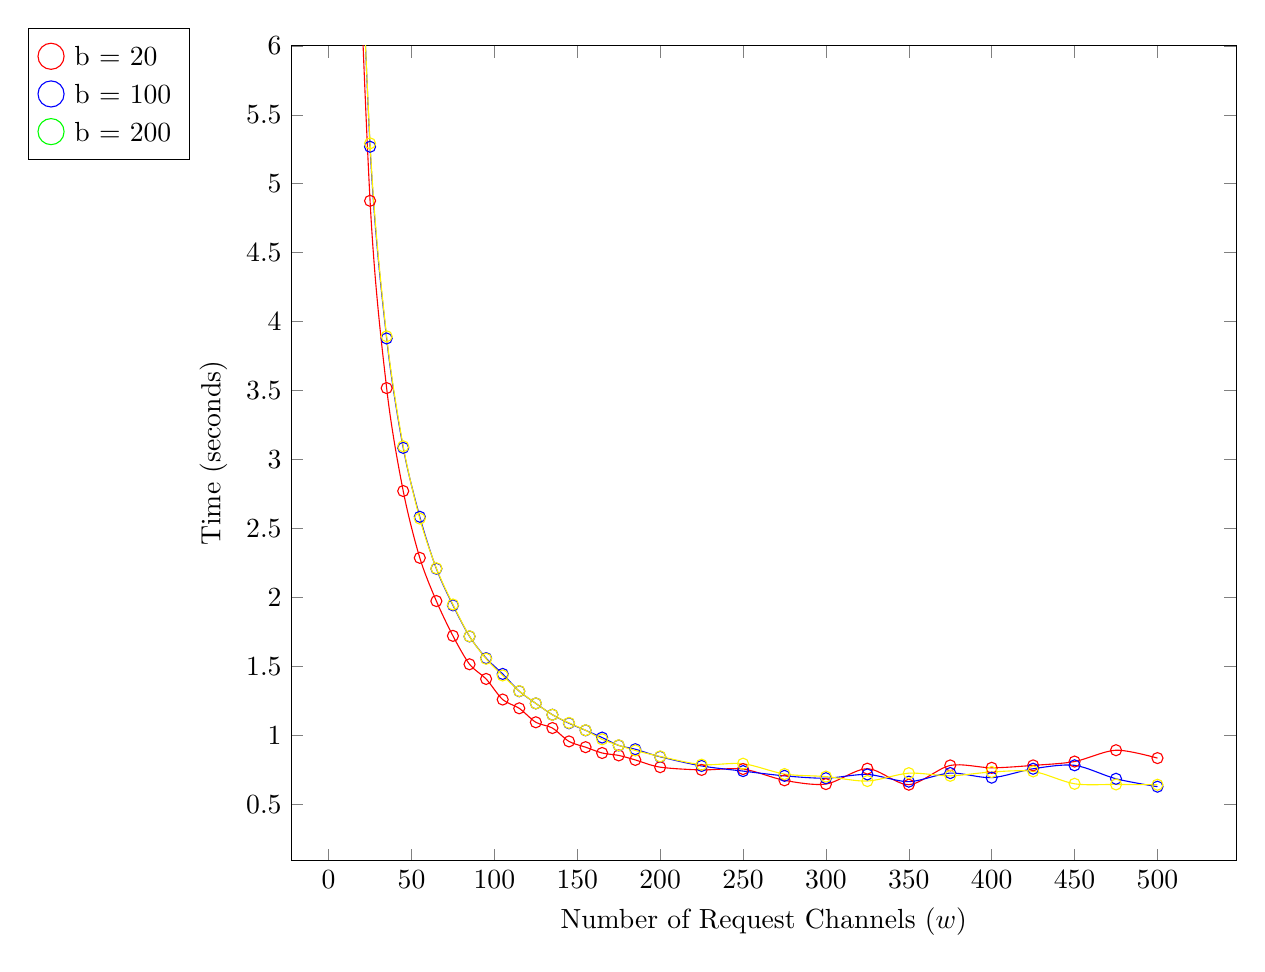
\begin{tikzpicture}[scale=1, transform shape]
\pgfplotsset{
    scale only axis,
}

	\begin{axis}[
		xlabel={Number of Request Channels ($w$)},
		ylabel={Time (seconds)},
		ymax=6,
		%xmode=log,
		%log basis y=10
	]
	\addplot[color=red,smooth,mark=o] coordinates {
(1,120.349)
(5,23.8298)
(10,11.9867)
(15,8.0388)
(25,4.87644)
(35,3.51912)
(45,2.77298)
(55,2.28876)
(65,1.97553)
(75,1.72314)
(85,1.51737)
(95,1.41106)
(105,1.2618)
(115,1.1982)
(125,1.09697)
(135,1.05527)
(145,0.958301)
(155,0.916554)
(165,0.874241)
(175,0.856789)
(185,0.824185)
(200,0.771622)
(225,0.751684)
(250,0.757913)
(275,0.67616)
(300,0.649102)
(325,0.760782)
(350,0.644573)
(375,0.78435)
(400,0.766926)
(425,0.78442)
(450,0.8123)
(475,0.894577)
(500,0.837287)
	};
	\addplot[color=blue,smooth,mark=o] coordinates {
(1,121.251)
(5,25.2386)
(10,12.1703)
(15,8.49767)
(25,5.26832)
(35,3.87888)
(45,3.08587)
(55,2.58636)
(65,2.20966)
(75,1.94459)
(85,1.71934)
(95,1.56183)
(105,1.44736)
(115,1.32203)
(125,1.23375)
(135,1.1517)
(145,1.08988)
(155,1.03858)
(165,0.986069)
(175,0.928991)
(185,0.901825)
(200,0.846869)
(225,0.780397)
(250,0.743195)
(275,0.70866)
(300,0.691533)
(325,0.718946)
(350,0.666577)
(375,0.728925)
(400,0.695512)
(425,0.760074)
(450,0.785047)
(475,0.687394)
(500,0.630089)
	};
	\addplot[color=yellow,smooth,mark=o] coordinates {
(1,123.139)
(5,24.4226)
(10,12.4222)
(15,8.46557)
(25,5.29297)
(35,3.89466)
(45,3.09731)
(55,2.57336)
(65,2.21331)
(75,1.95065)
(85,1.72055)
(95,1.55709)
(105,1.43616)
(115,1.3232)
(125,1.23387)
(135,1.15142)
(145,1.09268)
(155,1.03947)
(165,0.973288)
(175,0.930332)
(185,0.892551)
(200,0.849524)
(225,0.789965)
(250,0.796844)
(275,0.721709)
(300,0.70331)
(325,0.671004)
(350,0.727991)
(375,0.708938)
(400,0.73671)
(425,0.74085)
(450,0.651054)
(475,0.646474)
(500,0.644278)
	};
	\end{axis}
	
		\matrix [draw,below left] at (current bounding box.north west) {
  \node [style={draw = red,shape=circle},label=right:{b = 20}] {}; \\
  \node [style={draw = blue,shape=circle},label=right:{b = 100}] {}; \\
  \node [style={draw = green,shape=circle},label=right:{b = 200}] {}; \\
};
	
\end{tikzpicture}
\caption{Runtimes for $n = 10000$}
\end{figure}

Compared to PA4, this program runs a little bit faster since there is less overhead incurred by context switching threads. Increasing the number of request channels (\texttt{-w $n$}) still serves to improve performance up to a certain point. The best number of channels varies significantly based on the number of the size of the buffer. For small buffer sizes, around 275 channels is best, but with a large buffer, the best performance is attained with around 475 channels.

Beyond those numbers of channels, the program becomes slower again, since at that point the overhead of maintaining the state of all the channels outweighs the benefits that using multiple channels provides.

If the program spawns more than one worker thread, however, and splits up handling of channels between them, the program can benefit from as many as 1,000 channels. From my testing, the best number of threads is around half the number of physical CPU cores: 10 on my system.

\begin{table}[h]
\begin{tabular}{r|c|c|c}
\multicolumn{1}{c|}{\textbf{Worker Threads}} & \multicolumn{1}{c|}{\textbf{b=20}} & \multicolumn{1}{c|}{\textbf{b=100}} & \multicolumn{1}{c}{\textbf{b=200}} \\ \hline
1 & 120.349 & 121.251 & 123.139 \\
5 & 23.8298 & 25.2386 & 24.4226 \\
10 & 11.9867 & 12.1703 & 12.4222 \\
15 & 8.0388 & 8.49767 & 8.46557 \\
25 & 4.87644 & 5.26832 & 5.29297 \\
35 & 3.51912 & 3.87888 & 3.89466 \\
45 & 2.77298 & 3.08587 & 3.09731 \\
55 & 2.28876 & 2.58636 & 2.57336 \\
65 & 1.97553 & 2.20966 & 2.21331 \\
75 & 1.72314 & 1.94459 & 1.95065 \\
85 & 1.51737 & 1.71934 & 1.72055 \\
95 & 1.41106 & 1.56183 & 1.55709 \\
105 & 1.2618 & 1.44736 & 1.43616 \\
115 & 1.1982 & 1.32203 & 1.3232 \\
125 & 1.09697 & 1.23375 & 1.23387 \\
135 & 1.05527 & 1.1517 & 1.15142 \\
145 & 0.958301 & 1.08988 & 1.09268 \\
155 & 0.916554 & 1.03858 & 1.03947 \\
165 & 0.874241 & 0.986069 & 0.973288 \\
175 & 0.856789 & 0.928991 & 0.930332 \\
185 & 0.824185 & 0.901825 & 0.892551 \\
200 & 0.771622 & 0.846869 & 0.849524 \\
225 & 0.751684 & 0.780397 & 0.789965 \\
250 & 0.757913 & 0.743195 & 0.796844 \\
275 & 0.67616 & 0.70866 & 0.721709 \\
300 & 0.649102 & 0.691533 & 0.70331 \\
325 & 0.760782 & 0.718946 & 0.671004 \\
350 & 0.644573 & 0.666577 & 0.727991 \\
375 & 0.78435 & 0.728925 & 0.708938 \\
400 & 0.766926 & 0.695512 & 0.73671 \\
425 & 0.78442 & 0.760074 & 0.74085 \\
450 & 0.8123 & 0.785047 & 0.651054 \\
475 & 0.894577 & 0.687394 & 0.646474 \\
500 & 0.837287 & 0.630089 & 0.644278
\end{tabular}
\end{table}


\end{document}
